\documentclass{article}

% Language setting
\usepackage[english]{babel}
\usepackage{tikz}
\usetikzlibrary{shapes,arrows}
\usetikzlibrary{arrows.meta, positioning}

% Set page size and margins
\usepackage[letterpaper,top=2cm,bottom=2cm,left=3cm,right=3cm,marginparwidth=1.75cm]{geometry}

% Useful packages
\usepackage{amsmath}
\usepackage{graphicx}
\usepackage[colorlinks=true, allcolors=blue]{hyperref}

\title{Software Testing 2022/3 Portfolio}
\author{Guolong}

\begin{document}
\maketitle

\section{Outline of the Software Being Tested}

The software under test is a REST-based pizza-delivery system with two key endpoints:
\texttt{validateOrder} and \texttt{calcDeliveryPathAsGeoJson}.
\texttt{validateOrder} checks credit card details, pizza counts, and pricing constraints;
\texttt{calcDeliveryPathAsGeoJson} computes a drone route under no-fly-zone and central-area rules in GeoJSON.
The test approach employs boundary value analysis, scenario-based coverage,
and code instrumentation (e.g.\ JaCoCo) to ensure thorough validation of these endpoints
across both functional and technical quality criteria.\footnote{https:$//$github.com$/$GuolongTang111$/$ILP\_for\_ST\_CW containing source code and documents is provided.}

\section{Learning Outcomes}
\begin{enumerate}
    \item \textbf{Analyze requirements to determine appropriate testing strategies} \marginpar{[default 20\%]}
    \begin{enumerate}
        \item \textbf{Range of requirements, functional requirements, measurable quality attributes, qualitative requirements\footnote{For full requirements and models see ./ilp\_submission\_1/20241025 ILP CW2 Spec.pdf.}}
        \begin{itemize}
            \item \textbf{Functional:}
            The \texttt{validateOrder} endpoint accepts an order and returns \texttt{400} if it detects a valid or partially erroneous order, along with an \texttt{orderStatus} and \texttt{validationCode}.
            The \texttt{calcDeliveryPathAsGeoJson} endpoint receives a valid order, computes an array of drone poses for delivery and potential return, and internally performs validation. 
            If the order proves invalid, it also provides the \texttt{orderStatus} and \texttt{validationCode}. 
            \item \textbf{Quality Attributes:}
            The system focuses on performance metrics such as execution speed for \texttt{calcDeliveryPathAsGeoJson}, where lengthy distance path planning is measured against time thresholds.
            \item \textbf{Qualitative Attributes:}
            Robustness is verified by testing missing or malformed fields (e.g.\ incomplete orders), ensuring that the system gracefully identifies such deficiencies.
        \end{itemize}
    
        \item \textbf{Level of requirements, system, integration, unit}
        \begin{itemize}
            \item \textbf{System-Level:}
            System tests operate in Docker and mimic realistic usage, as the submitted image runs under an autograder or similar environment.
            \item \textbf{Integration-Level:}
            Integration tests concentrate on interactions among methods, such as linking external databases with the endpoints. 
            \item \textbf{Unit-Level:}
            Unit tests focus on isolated functions (e.g.\ verifying credit-card checks, route submethods) in a controlled setting, ensuring each component’s correctness.
        \end{itemize}
        
        \item \textbf{Identifying test approach for chosen attributes}
        \begin{itemize}
            \item \textbf{Functional Testing:}
            Both black-box (input-output matching) and white-box (code-level checks) strategies ensure correctness. 
            Tests are automated for most scenarios, while GeoJSON path correctness may include manual verification of complex route structures.
            \item \textbf{Performance and Coverage:}
            The \texttt{calcDeliveryPathAsGeoJson} integration test fails if response time exceeds five seconds. 
            Approximately 600 system-level calls test stability and detect missing fields in orders (robustness). 
            JaCoCo measures code coverage, focusing on critical logic paths and boundary conditions.
        \end{itemize}
    
        \item \textbf{Assess the appropriateness of the chosen testing approach}
        The overall approach (functional, performance, robustness) aligns well with the specification’s requirements, and TDD fosters early detection of defects. 
        However, in line with the marking scheme, certain areas are not covered, such as multiple concurrent errors in \texttt{validateOrder}, security tests (SQL injection or data leaks), or exhaustive no-fly corner cases. 
        These omissions may indicate a less comprehensive scope than an industry-level system. 
        Nevertheless, the approach remains effective for typical academic workloads; awarding a higher mark would require stronger evidence of additional coverage (e.g.\ concurrency, security, advanced performance analysis).
        \begin{itemize}
            \item \textbf{Potential Gaps:}
            All \texttt{validateOrder} test scenarios contain at most one error. 
            No security checks are present, leaving sensitive credit-card data untested for injection or misuse scenarios. 
            Edge no-fly zones and invalid-path conditions remain partly unexplored. 
            Network fetch failures (e.g.\ external dependencies) are not examined, highlighting a gap in resilience testing.
        \end{itemize}
    \end{enumerate}

\item \textbf{Design and implement comprehensive test plans with instrumented code} \marginpar{[default 20\%]}
\begin{enumerate}
\item \textbf{Construction of the test plan \footnote{For graphical illustration see Appendix. Fig.1}:}
A Test-Driven Development (TDD) approach underpins the construction of the test plan, ensuring
that new tests are created or adapted before implementing each corresponding requirement.
Early on, a basic set of tests mapped to core needs (e.g.\ credit-card checks in \texttt{validateOrder}),
and as additional functionality emerged (e.g.\ further route constraints in \texttt{calcDeliveryPathAsGeoJson}),
the test set expanded to accommodate performance targets and route-validation scenarios.
For instance, upon deciding to verify outstanding order details or route constraints, the system-level
tests were adjusted to confirm both correctness and speed under normal loads. In practice,
integration and system tests also include certain manual checks, due to the extensive JSON outputs
and the challenge of preparing automated reference data. Relevant documentation (e.g.\ coverage
reports, time measurements) is updated alongside each newly introduced requirement, demonstrating
how the test plan evolves to meet both functional and performance criteria throughout the project. 

\item \textbf{Evaluation of the quality of the test plan:}
The test plan systematically mapped each requirement to dedicated test scenarios, ensuring
that no-fly compliance and credit-card validations were covered. Code instrumentation
(e.g.\ asserts, diagnostic logging) was used to detect boundary issues early, such as borderline
polygons or malformed orders. This enabled quick feedback for functional errors in route
computations and pizza constraints. However, multi-thread scenarios and concurrency testing
were largely unaddressed, limiting insights into potential race conditions. Furthermore,
while performance was briefly measured within Docker-based tests, extended soak or stress
testing was not pursued. The instrumentation itself was somewhat ad hoc, relying on manual
log checks rather than a consistent tool-based approach. Overall, the plan ensured core
coverage but left some gaps in concurrency robustness and automated performance tracking.

\item \textbf{Instrumentation of the code:}
Targeted diagnostic checks and logging statements were inserted throughout the \texttt{OrderValidationService}
and \texttt{DeliveryPathService} classes to reveal boundary issues and failure modes quickly.
For example, in \texttt{validateOrder}, an \texttt{assert} confirmed credit-card 
fields were non-null before parsing (\texttt{commit \#a47c1}), while debug-level logs in the drone path
computation code captured whether a segment intersected a no-fly polygon
(\texttt{DronePathCalculator.java}, line 112). These checks permitted early detection
of borderline route errors without needing a large external harness. JaCoCo instrumentation
also measured coverage to verify exercised branches and lines. However, instrumentation
remained somewhat localized, using logs and asserts at key points rather than a standardized
logging framework. This still proved beneficial for detecting issues (e.g.\ missing GeoJSON
properties) and guiding further expansions.

\item \textbf{Evaluation of the instrumentation:}
Overall, instrumentation provided sufficient visibility into common failures, 
such as invalid credit-card inputs or no-fly-zone edge cases. By adding targeted asserts
and debug logs, borderline errors were caught quickly without excessive overhead. However,
ad hoc instrumentation can complicate uniform log parsing, and no dedicated timestamping
was implemented for route calculations or credit-card checks. A more systematic approach,
such as a logging framework with consistent trace IDs, would enhance traceability and
automated analysis. Nevertheless, the current instrumentation covers primary validation
and pathfinding concerns effectively.
\end{enumerate}

\item \textbf{Apply a wide variety of testing techniques and compute test coverage and yield according to a variety of criteria} \marginpar{[default 20\%]}
\begin{enumerate}
\item\textbf{Range of techniques:}
A mix of functional API tests (e.g.\ verifying each error code for \texttt{validateOrder}),
performance checks (timing \texttt{calcDeliveryPath} calls under varying load), and Docker-based
integration tests was employed. These approaches addressed correctness, speed,
and resilience to malformed input. Although no full-scale stress tests were conducted, limited
parallel-request tests confirmed that the endpoints remain responsive under modest demand.

\item\textbf{Evaluation criteria for the adequacy of the testing:}
Line coverage (via JaCoCo) was combined with scenario-based validation (ensuring all major error
codes were triggered in distinct test cases). Achieving high coverage in pathfinding classes was
essential for validating route generation logic. Time-based thresholds (from the specification's
performance buckets) further ensured that the suite addressed both functional correctness
and efficiency.

\item \textbf{Results of testing:}
Final test runs revealed near-complete line coverage in \\\texttt{OrderValidationService} (98\%)
and in the drone path modules (97\%),\footnote{Full coverage reports reside at 
\texttt{./ilp\_submission\_1/target/site/jacoco/index.html}.}
while performance timings placed route computation into the second-fastest group.
Each major error code (e.g.\ \texttt{CARD\_NUMBER\_INVALID}, \texttt{PIZZA\_COUNT\_EXCEEDED}) 
was validated by scenario-based tests, and Docker-based end-to-end checks detected no
unexpected failures.

\item \textbf{Evaluation of the results:}
These coverage and scenario outcomes suggest that key requirements (validation, path logic,
GeoJSON output) are well tested, though corner cases (extremely large orders or prolonged
no-fly segments) remain partially addressed. Nonetheless, strong coverage and scenario diversity
provide confidence in correctness and performance under moderate loads. Extended stress tests
or mutation testing could further clarify residual fault levels.
\end{enumerate}

\item \textbf{Evaluate the limitations of a given testing process, using statistical methods where appropriate, and summarise outcomes} \marginpar{[default 20\%]}
\begin{enumerate}
\item \textbf{Identifying gaps and omissions in the testing process:}
The existing tests center on endpoint correctness and moderate performance scenarios. 
Extremely large no-fly data, concurrency, or heavy parallel load scenarios have not been thoroughly tested, 
and structured availability checks under parallel requests are lacking.

\item \textbf{Identifying target coverage/performance levels for the different testing procedures:}
The initial goal was at least 85\% coverage in validation logic and 80\% in pathfinding,
along with the second-fastest performance tier. 

\item \textbf{Discussing how the testing carried out compares with the target levels:}
Coverage surpassed 90\%, outdoing the original 85\% aim. 
Route-computation speed met second-tier speed thresholds,
but concurrency and resilience objectives were left undefined.

\item \textbf{Discussion of what would be necessary to achieve the target level:}
A short stress suite (potentially mutation-based) could quantify residual faults.
Explicit concurrency benchmarks (e.g.\ 20 parallel requests) might strengthen confidence in 
peak-load reliability. Such steps would help validate real-world conditions and fill the
gaps in concurrency and advanced performance checks.
\end{enumerate}

\item \textbf{Conduct reviews, inspections, and design and implement automated testing processes} \marginpar{[default 20\%]}
\begin{enumerate}
\item \textbf{Identify and apply review criteria to selected parts of the code and identify issues in the code}
Code reviews targeted areas like \texttt{OrderValidationService} and \texttt{DronePathCalculator} 
for clarity (naming, structure) and correctness (no-fly logic, input checks). 
Discrepancies in borderline credit-card validations were unified based on peer feedback.
A complex route method was also refactored for improved readability.

\item \textbf{Construct an appropriate CI pipeline for the software\footnote{For CI execution history, see the repository's Actions tab}}
A GitHub Actions pipeline checks out the repository, builds a Docker image, runs Maven-based unit and integration tests, 
then executes a Postman test suite for each endpoint. Logs and test artifacts are retained to ensure transparency. 
This mirrors common DevOps patterns, requiring each commit to be validated automatically.

\item\textbf{Automate some aspects of the testing}
Scenario-based checks (e.g.\ credit-card error codes, path correctness) are automated via Newman (Postman CLI). 
Docker-based containers confirm end-to-end system health, while JaCoCo coverage data is collected automatically. 
Hence, essential tests run with minimal manual intervention.

\item \textbf{Demonstrate the CI pipeline functions as expected}
Each push triggers a build–test cycle, failing if \texttt{validateOrder} or route computations do not pass. 
Coverage below 80\% for critical classes raises warnings. Consequently, the pipeline consistently identifies 
defects early and confirms partial performance metrics, aligning with the specified requirements.
\end{enumerate}
\end{enumerate}

\appendix{}
\section{Figures}
\begin{figure}[htbp]
    \scalebox{0.75}{
    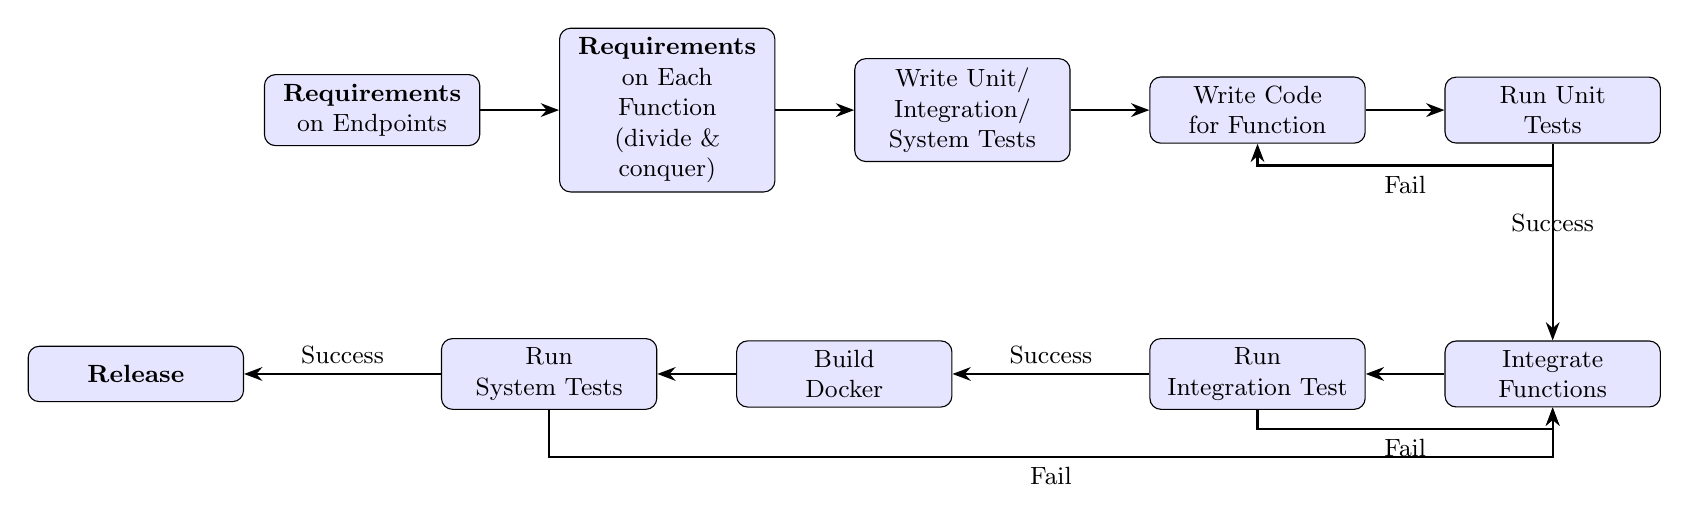
\begin{tikzpicture}[
        font=\small,
        node distance=1cm,
        >=Stealth,
        line/.style={->, thick},
        process/.style={rectangle, draw, rounded corners,
          align=center, fill=blue!10, minimum height=2em,
          text width=2.5cm},
        decision/.style={diamond, draw, aspect=1.4, align=center,
          fill=red!10, inner sep=0pt, text width=2cm}
    ]
    
    %--- NODES ---
    \node[process] (reqend) {
      \textbf{Requirements}\\
      on Endpoints
    };
    
    \node[process, right=of reqend] (reqfunc) {
      \textbf{Requirements}\\
      on Each Function\\
      (divide \& conquer)
    };
    
    \node[process, right=of reqfunc] (testreq) {
      Write Unit/\\
      Integration/\\
      System Tests
    };
    
    \node[process, right=of testreq] (writefunc) {
      Write Code\\
      for Function
    };
    
    \node[process, right=of writefunc] (unittest) {
      Run Unit\\
      Tests
    };
    
    \node[process, below=2.5cm of unittest] (integrate) {
      Integrate\\
      Functions
    };
    
    \node[process, left=of integrate] (inttest) {
      Run\\
      Integration Test
    };
    
    \node[process, left=2.5cm of inttest] (docker) {
      Build\\
      Docker
    };
    
    \node[process, left=of docker] (systest) {
      Run\\
      System Tests
    };
    
    \node[process, left=2.5cm of systest] (release) {
      \textbf{Release}
    };
    
    %--- CONNECTIONS (ARROWS) ---
    \draw [line] (reqend) -- (reqfunc);
    \draw [line] (reqfunc) -- (testreq);
    \draw [line] (testreq) -- (writefunc);
    \draw [line] (writefunc) -- (unittest);
    
    % If unit tests fail
    \draw [line] (unittest) |- ++(0,-2em) -| node[near start, below]{Fail} (writefunc);
    % If success
    \draw [line] (unittest) -- node[above]{Success} (integrate);
    \draw [line] (integrate) -- (inttest);
    % If integration fails
    \draw [line] (inttest) |- ++(0,-2em) -| node[near start, below]{Fail} (integrate);
    % If success
    \draw [line] (inttest) -- node[above]{Success} (docker);
    \draw [line] (docker) -- (systest);
    % If system fails
    \draw [line] (systest) |- ++(0,-3em) -| node[near start, below]{Fail} (integrate);
    % If success
    \draw [line] (systest) -- node[above]{Success} (release);
    
    \end{tikzpicture}
    }
    \caption{Test-driven development flow}
\end{figure}

\end{document}
